\documentclass[10pt,conference,a4paper]{IEEEtran}
\usepackage[utf8]{inputenc}
\usepackage[T1]{fontenc}
% Correct date format in references but with american hyphenation, quotes, ...
% Trick from http://tex.stackexchange.com/a/129209
\usepackage[australian,american]{babel}

% *** GRAPHICS RELATED PACKAGES ***
\ifCLASSINFOpdf
  \usepackage[pdftex]{graphicx}
\else
  \usepackage[dvips]{graphicx}
\fi

% *** MATH PACKAGES ***
\usepackage{amssymb}
\usepackage[cmex10]{amsmath}

% Figure captions in small font
\makeatletter
\let\MYcaption\@makecaption
\makeatother
\usepackage[font=footnotesize]{subcaption}
\makeatletter
\let\@makecaption\MYcaption
\makeatother

\usepackage{pgfplots}
\pgfplotsset{compat=1.9}
%TODO minted ?
\usepackage[binary-units]{siunitx}
\usepackage{booktabs}
\usepackage{pifont}
\usepackage{tikz}
\usepackage{csquotes}
\usepackage[backend=biber,style=ieee,minbibnames=1,maxbibnames=3]{biblatex}
\usepackage{url}
\usepackage[backgroundcolor=lightgray]{todonotes}
\usepackage[hidelinks]{hyperref}

\bibliography{paper}
% Small font for references
\renewcommand*{\bibfont}{\small}

% correct bad hyphenation here
\hyphenation{op-tical net-works semi-conduc-tor}

% paper title
% can use linebreaks \\ within to get better formatting as desired
\def\mytitle{EpTO: An Epidemic Total Order Algorithm for Large-Scale Distributed Systems}
\title{\mytitle}

% author names and affiliations
% use a multiple column layout for up to three different
% affiliations
\def\jocelyn{Jocelyn Thode}
\def\ehsan{Ehsan Farhadi}
\author{\IEEEauthorblockN{\jocelyn\IEEEauthorrefmark{1},
\ehsan\IEEEauthorrefmark{2}}
\IEEEauthorblockA{Université de Neuchâtel\\
Neuchâtel, Switzerland\\
Email: \IEEEauthorrefmark{1}\href{mailto:jocelyn.thode@unifr.ch}{jocelyn.thode@unifr.ch},
\IEEEauthorrefmark{2}\href{mailto:ehsan.farhadi@unine.ch}{ehsan.farhadi@unine.ch}}}

% Set PDF file properties
\hypersetup{
	pdftitle=\mytitle,
}

% Tick marks
\newcommand{\cmark}{\ding{51}}
\newcommand{\xmark}{\ding{55}}

% Columns balancing
\renewbibmacro{finentry}{%
  \iffieldequalstr{entrykey}{jujjuri2010virtfs}%<- key after which you want the break
   {\finentry\newpage}
   {\finentry}}

\begin{document}
\graphicspath{{figures/}}


% make the title area
\maketitle


\begin{abstract}
One of the fundamental problems of distributed computing, is the ordering of events through all peers. From all the available orderings, total ordering is of particular interest as it provides a powerful abstraction for building reliable distributed applications. unfortunately, existing algorithms can not provide reliability, scalability, resiliency and total ordering in one package. EpTO is a total order algorithm with probabilistic agreement that scales both in the number of processes and events. EpTO provides deterministic safety and probabilistic liveness: integrity, total order and validity are always preserved, while agreement is achieved with arbitrarily high probability. We are going to implement EpTO using the NeEM library and show EpTO is well-suited for large-scale dynamic distributed systems, and afterwards we will evaluate this algorithm by comparing it with currently being used ordering algorithms.
\end{abstract}

\section{Introduction}
The ordering of events is one of the most fundamental problems in distributed systems and it has been studied over past few decades. A lot of researchers have been working on an algorithm with different guarantees and trade-offs such as synchronization, agreement or state machine replication \todo{Cite papers}
. But because these properties are strong guarantees, the algorithms that implements them do not scale very well. Existing probabilistic protocols are highly scalable and resilient, but they can not provide total ordering in large scale distributed systems, and existing deterministic protocols which provide total ordering, are not resilient and are scalable.
\par
The problem with existing deterministic total ordering protocols, is that they need some sort of agreement between all peers in the system on the order of messages. This causes a massive amount of network traffic and overhead on the system.
Moreover, an agreement feature for an asynchronous system requires to
explicitly maintain a group and have access to a failure detector. Due to the faults and churn in large-scale distributed systems, failure detector turns into bottleneck of the system and thus, limits scalability of the algorithm.
\subsection{Contribution}
EpTO \autocite{matos2015epto} guarantees that processes eventually agree on the set of received events with high probability and deliver these in total order to the application. The intuition behind EpTO is that events are available quickly at all nodes with high probability,
Once events are thought to be available in every peer, each peer deterministically order them using the timestamp of each event and breaking ties with the id of the broadcaster peer, deliver them to the application accordingly.
\par
The main insight behind EpTO dissemination protocol is a \textit{balls-and-bins} approach. The \textit{balls-and-bins} problem is a basic probabilistic problem: consider \textit{n} balls and \textit{m} bins where we consequently throw balls into a bin, completely random and independent from other balls.
\par
A balls-and-bins approach abstracts peers as bins and messages (events) as balls, and studies how many balls need to be \textit{thrown} such that each bin contains at least one ball with arbitrarily high probability \autocite{Koldehofe02simplegossiping}. Using this approach the number of messages transmitted per process per round is logarithmic in the number of processes, and the total number of messages
transmitted in the network before an event is delivered is low and uniform over all peers.


\begin{figure}
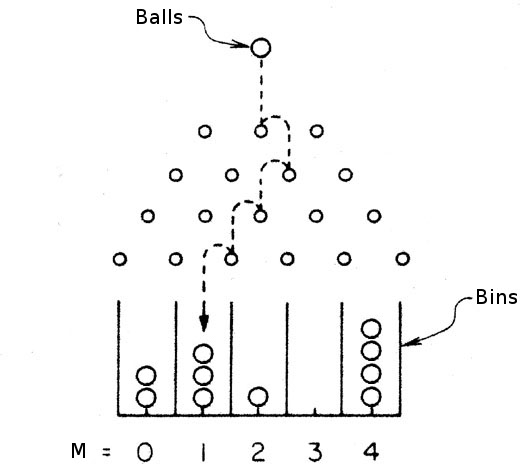
\includegraphics[width=\linewidth]{figures/BnB.jpeg}
\caption{Balls-and-Bins}
\label{fig:balls-and-bins}
\end{figure}
\par
In this paper, we will implement EpTO and compare it against a known deterministic total order algorithm, namely JGroups \autocite{jgroups}.

These tasks will be split in two tasks. The first task will assume that all peers are known by all peers. We will implement EpTO using this assumption and test it against JGroups. The second task will assume unknown membership on all peers. We will update EpTO and use a PSS\footnote{Peer Sampling Service}. We will also update the underlying layer NeEM \autocite{neem} to use UDP instead of TCP and switch to NIO.2\footnote{Non-blocking I/O available from Java 7}.

\section{Ordering Algorithms}
\todo[inline]{We will explain why Ordering algorithms are necessary, the difference between partial order and Total order and why partial order might not be sufficient in some cases}

Distributed systems, like centralized systems need to preserve the temporal order of event produced by concurrent process in the system. When there are separated processes that can only communicate through messages, you can’t easily order these messages.
Therefore we need ordering algorithms to overcome this problem.
\par
We have two types of ordering algorithms \autocite{lamport1978time}: the partial order algorithms and the total order algorithms.
\subsection{Partial Order Algorithms}
Assuming S is partially ordered under $\leq$, then the following statements hold for all a, b and c in S:
\begin{itemize}
	\item Reflexivity: $a \leq a$ for all $a \in S$.
	\item Antisymmetry: $a \leq b$ and $b \leq a$ implies $a=b$ .
	\item Transitivity: $a \leq b$  and $b \leq c$  implies $a \leq c$.
\end{itemize}

\subsection{Total Order Algorithms}
A totally ordered set of events is a partially ordered set which satisfies one additional property:
\begin{itemize}
	\item Totality (trichotomy law): For any $a, b \in S$, either $a \leq b$  or $b \leq a$.
\end{itemize}
\todo[inline]{Explain advantages and usefulness of both systems}


\section{EpTO}
\begin{figure}
	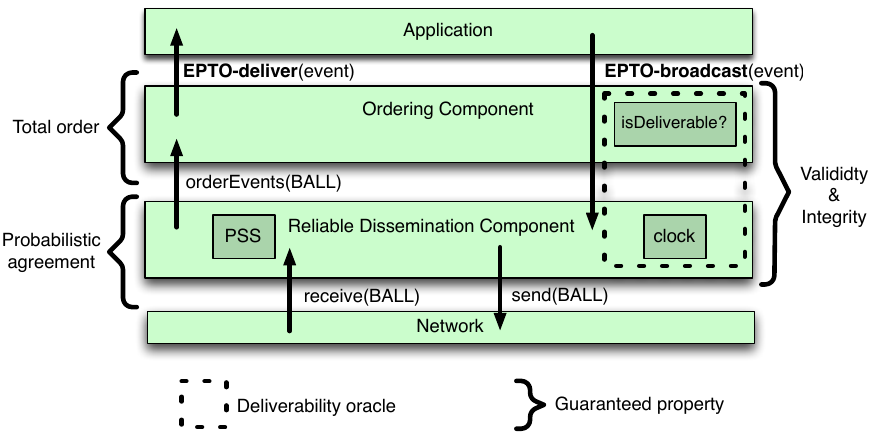
\includegraphics[width=\linewidth]{figures/epto-architecture.png}
	\caption{\todo[inline]{We need a better quality figure (SVG)}\protect\footnotemark{}.}
	\label{fig:epto-architecture}
\end{figure}
\subsection{Definitions}
A process or peer is defined as an actor in our system running the application that needs total order. Each process will communicate with other processes in the distributed systems and exchange events and order them together.
\par
An event is defined as something that happens at a given time. For example, we could imagine a system where each process publish some sort of data. The moment where this data is published combined with the data is called an event.
\par
A ball is a set of events bundled together and sent as one package. We use balls in EpTO to reduce network traffic and make it scalable in terms of processes and events.

EpTO is scalable in the sense that \todo[inline]{Explain the logarithmic scalability}

\par
Since EpTO is using a probabilistic agreement instead of a deterministic agreement, there might be a situation where a peer does not receive an event (with a very low arbitrary probability). In this case there will be a hole in the sequence of delivered events but even in this case, the order of the delivered event will be protected by EpTO's deterministic ordering algorithm and total order property is preserved.
\subsection{Dissemination Component}
The Dissemination component is the component that bridges EpTO with the rest of the network. As we can see in Figure \ref*{fig:epto-architecture}, it is in charge of receiving balls, open them , pass them to the Ordering component and then forward them to \textit{K} other processes, where K denotes the gossip fan-out.
\par
When an application wants to publish an event, it will broadcast this event to the Dissemination component.

\subsection{Ordering Component}
The Ordering component is responsible for ordering events before delivering them to the application.
To achieve this, the Ordering component has a \textit{received} hash table of (\textit{id}, \textit{event}) pairs containing all the events which are received by the peer, but not yet delivered to the application and a \textit{delivered} hash table containing all the events which are delivered.
\par
In brief, the Ordering component first increments the timestamp of all the events which have been received in previous rounds to indicate the start of a new round. Then, it processes new events in the received ball by discarding events that have been received already (delivered events or events with timestamp smaller than the last delivered event). This is done to prevent delivering duplicate events. The remaining events in the received ball will be added to the \textit{received} hash table, and wait to be delivered based on the Stability oracle.
\subsection{Stability Oracle}
The Stability oracle is the component that outputs timestamps. It will increment its local clock every round as well as synchronize itself using timestamps of newly received events, to make sure the local clock does not drift too much.
\par
This Stability oracle offers an API to the Ordering component letting it know when an event is mature enough to be delivered to the application.
\par
As this component is local and only correct itself when we receive new events, it generates no network traffic. This means it does not impact the scalability of EpTO.
\section{Performance Comparisons}
\todo[inline]{Here we will present the different test we ran, the methodology used and the result we obtained}
\subsection{Methodology}
\todo[inline]{Here we explain how we ran our tests and on what type of machines}
\subsection{Peer membership known}
\todo[inline]{We will present the results obtained and try to explain the results}
\subsection{Peer membership unknown}
\todo[inline]{We will present the results obtained and try to explain the results}

\section{Conclusion}
\todo[inline]{He we will summarize the results we found and present some future tasks that could be accomplished on EpTO}


% conference papers do not normally have an appendix


% use section* for acknowledgement
\section*{Acknowledgment}
\todo[inline]{Write acknowledgment}




% references section, with correct date format
\begin{otherlanguage}{australian}
\printbibliography
\end{otherlanguage}

% that's all folks
\end{document}
